%%%%%%%%%%%%%%%%%%%%%%%%%%%%%%%%%%%%%%%%%%%%%%%%%%%
%
%  New template code for TAMU Theses and Dissertations starting Spring 2021.  
%
%
%  Author: Thesis Office
%  
%  Last Updated: 1/13/2021
%
%%%%%%%%%%%%%%%%%%%%%%%%%%%%%%%%%%%%%%%%%%%%%%%%%%%

%%%%%%%%%%%%%%%%%%%%%%%%%%%%%%%%%%%%%%%%%%%%%%%%%%%%%%%%%%%%%%%%%%%%%%%
%%%                           SECTION II (IX - this is a section II re-write)
%%%%%%%%%%%%%%%%%%%%%%%%%%%%%%%%%%%%%%%%%%%%%%%%%%%%%%%%%%%%%%%%%%%%%%


\chapter{\MakeUppercase{Literature Review}}
\label{cha:literature-review}

A review of the literature surrounding information quality research within market monitoring units signals that there is room for improvement in how value is generated from information assets. This gap is highlighted by several major issues (introduced in Chapter \ref{cha:Introduction} and discussed in this literature review), including:

\begin{enumerate}
    \item {Development of technology surrounding domain-specific language engineering}
    \item {An aging workforce in the electric utilities industry that is reaching the tipping point for replacement}
    \item {A lack of existing research on data and information quality within the market monitoring sphere}
    \item {A disruption of traditional energy market design due to advances in technology and the energy regulatory landscape}
\end{enumerate}

\noindent These issues represent a unique opportunity to obtain important value from the data assets both generated and used by professionals in the market monitoring sphere. The researcher will discuss each of these issues in the context of relevant literature\footnote{Appendix \ref{appendix:B} contains a listing of different search phrases used for locating relevant research discussed in this chapter.},
and then introduce possible sources of data that enable the development of a domain-specific language for market monitors.% ecg0122 - commenting this out since I rearranged these sections based on Dr. Berleant's recommendation indicate how this design science project has the potential to improve these issues within market monitoring.

\section{An Aging Workforce}

Many technical industries are experiencing the problem of an aging workforce; trained professionals are reaching retirement age at a rate faster than that of replacement. A 2006 study showed that the largest staff segment, of a surveyed group of energy professionals, is at (or beyond) retirement age. This same study cited "retirements, restructuring, and technology changes" as being the primary drivers of staff leaving the energy profession \cite{raysnyder}. Given the age of this study, many industries are currently going through a period of training new career professionals. Such a problem impacts market monitoring as well. 

MMUs (as previously discussed) were cemented into operation by the US federal government, not long before that same 2006 study. An energy research lab at UC Berkeley shows that staffing across market monitoring groups is relatively low compared to other organizations in the industry. According to Goldman, Lesieutre, and Bartholomew, all operational market monitoring groups in the US had fewer than 20 FTEs (each) in employ by 2004 \cite{goldman}.

While these numbers appear low in comparison to other organizations with energy industry staff\footnote{As of Q1 2025, Southwest Power Pool employs over 800 FTEs (including their internal market monitoring staff).}, this study declares that budgets and headcount (at that time) increased significantly for market monitoring work. As such, this shows a trend of growing demand for market monitoring staff in a workforce that, holistically, employs many individuals on (or beyond) the horizon of retirement. One claim to helping combat this "brain drain" problem is a technology framework that "facilitates knowledge retention" \cite{raysnyder}, including systems (supported by an IT organization) that capture necessary process knowledge.

\subsection{The Importance of Institutional Knowledge}

Given that the energy industry faces career professionals heading into retirement, this research intends to use a domain-specific language-based system to help preserve the institutional knowledge that is lost when market monitors retire (or even simply change positions). As employees make career transitions, the institutional knowledge that they built often leaves with them. In market monitoring, this problem is amplified due to two salient facts: 1) the number of individuals that work in market monitoring is small compared to the rest of the energy and utilities industries, and 2) market monitors often specialize in regards to analysis or policy work. Individuals who primarily work in market surveillance may never directly work in policy development (or vice-versa).

In a personal anecdote, this "brain drain" problem has been seen within the SPP MMU. Several long-term employees have exited the MMU in pursuit of other roles, only to leave undocumented code behind them that others must support. This code exists in the form of SQL queries and/or SAS scripts that contain embedded business rules (as they were understood by these employees). Deciphering and supporting this code becomes a burden for others that inherit the work of these departed employees.

A 2016 publication \textit{Knowledge Management in Esoteric Management} summarizes this issue well: "...knowledge sharing should be encouraged by placing employees working together closely to create pooled expertise..." \cite{knowledge-management-in-esoteric-management}. When employees share knowledge, they can keep important information from being destroyed when key individuals leave a department. One of the goals for the system that this dissertation designs is to foster knowledge sharing amongst employees.

\subsection{Application to Market Monitoring Research}

%As the previously discussed examples exhibit, 

Domain-specific programming languages (DSLs) are powerful interfaces that enable subject-matter experts (SME), in any particular domain of expertise, to perform tasks similar to a proper software developer that builds applications in general-purpose languages (GPL). A well-defined DSL can save many hours of development time for specific groups that have IT oriented needs. DSLs also have the ability to lower the "barriers to entry" for SMEs that wish to write applications to handle work within their purview. With support from a DSL, a software engineer does not need to be deeply involved in business rules to understand how to develop an application (a common issue in the energy industry). Likewise, SMEs do not need to heavily codify their business rules into software requirements for an application to be developed when utilizing a domain-specific language.

Following the theme of how DSLs are able to abstract away complexity of big data processing tasks, this research aims to bring such a tool set to bear on tasks performed in energy market monitoring. Commands embedded into a domain-specific language have the potential to speed up many repetitive tasks in the market monitoring domain, especially regarding the generation of report and stakeholder presentations.

\section{An Analysis of Domain-Specific Languages}

Consider programming languages on a spectrum from general purpose languages (GPLs) at one end to domain-specific languages (DSLs) on the opposite end \cite{tomaz-dsl}.\footnote{Kosar, Tomaz, et al. indicate the "schism" between the two languages by discussing that "GPLs tend to be general, resulting in
poor support for domain-specific notation \cite{tomaz-dsl}."}
DSLs are languages that are limited in purpose, scope, and grammar. Rather than supporting a programming language that can be utilized for constructing almost anything (as GPLs do), DSLs are created to solve issues within a single problem domain.

\begin{table}[ht]
    \centering
        \begin{tabular}{|p{6cm}|p{4cm}|p{4cm}|p{2cm}|}
        \hline
        %https://aws.amazon.com/what-is/sql/
        \textbf{Language} & \textbf{Supporting \newline Enterprise} & \textbf{Problem Domain} & \textbf{Paradigm} \\
        \hline
        Structured Query Language (SQL) & Various & Data Retrieval & Declarative \\
        \hline
        %https://developer.hashicorp.com/terraform/intro
        Terraform / HCL & Hashicorp & Cloud Infrastructure \newline Deployment & Declarative \\
        \hline
        %https://pig.apache.org 
        Apache Pig ("Pig Latin") & Yahoo / Apache \newline Software Foundation & Data Retrieval \newline \& Processing & Declarative \\
        \hline
        %https://dev.to/jpmcb/awk-a-beginners-guide-for-humans-3l25
        awk & Bell Labs (originally) & Text Processing & Procedural \\
        \hline
        \end{tabular}
    \caption{Selection of Well-Known Domain-Specific Languages}
    \label{tab:well-known-dsl}
\end{table}

\textit{Structured Query Language (SQL)} \cite{dsl-aws} is one such example of a DSL. SQL queries are designed to retrieve data from databases for extraction, reference, and analysis. SQL dialects have been designed to interface across a broad range of database management systems (for example: PL/SQL for Oracle or T-SQL for Microsoft SQL Server databases).

\textit{Terraform (HCL)} \cite{dsl-terraform}, a product of Hashicorp Corporation, is yet another example of a domain-specific language that is prevalent among cloud-based companies. Terraform is known as an "infrastructure-as-code" language, used to interact with numerous cloud platform providers (e.g. Amazon Web Services) to quickly deploy, scale, and spin-down cloud resources. Instead of requiring an engineer to use a console environment to configure cloud resources, that same engineer can write a set of scripts that will precisely configure and deploy all of their desired infrastructure at once.

\textit{Apache Pig} \cite{dsl-pig-latin} (and its associated programming language \textit{"Pig Latin"}) is also a DSL. Like SQL, it is a declarative language used for data retrieval and data processing. Developers at Yahoo created Pig as a way to abstract some of the complexity of SQL away from analysts who were working with large datasets. With fewer lines of code, an analyst could use Pig to parse and load a dataset into memory, perform processing tasks, and format and report the results. This was specifically useful to analysts processing large datasets because Pig was designed to take advantage of the high-performance computing facilities of Hadoop.

Yet another powerful example of DSLs can be seen in the ubiquitous Unix program: \textit{awk} \cite{dsl-awk}. Originally created by Unix developers Aho, Weinberger and Kerninghan\footnote{The name "awk" is an acronym formed from the first letters of the developer's last names.}, awk is a scripting language designed to process textual data--- one line at a time. The power of this systems allows individuals to write expressions that are simple to understand, efficient, and portable across different Linux implementations. Countless developers (including the author of this dissertation) have made use of awk's utilities to process and format data in a headless environment.

Each of the languages represented in this review are, on their own, infeasible for writing general purpose applications. SQL, for example, should not be used to write a desktop program. They were, instead, each created to solve specific issues within their respective problem domains. Likewise, Terraform cannot be used to create web applications or develop billing software. One of the "upsides" of these languages are that they can quickly handle tasks within a specific problem domain.

\subsection{DSL Variations}

Each of the language examples provided here share a common characteristic in that they are external DSLs. They are interpreted and executed by a runtime program. This trait of DSLs separates them from another subset of domain-specific languages: internal DSLs. These are embedded langauges (sometimes referred to as fluent interfaces) that rely on a (usually) general-purpose language to parse their individual syntactic structures and execute logic. These DSL features are sometimes referred to as \textit{syntactic sugar} \cite{syntactic-sugar}, implying that they make the experience of developing solutions in them "sweeter" than without them.

Another common characteristic of DSLs lies in the fact that they are often text-based programming environments. As discussed later in this literature review, graphical domain-specific languages also exist. These are usually seen in the form of either enterprise extract-transform-load (ETL) applications or language workbenches. Jetbrains MPS is a prominent example of the power of graphical DSL representations. Business users are usually positioned to take advantage of these product offerings because they pose abstract interfaces (environments that allow users to graphically model \textit{what they want} instead of having to explicitly write source code in a general purpose language). With basic instruction, users can string together components that construct repeatable workflows without requiring them to possess deep programming knowledge.

\section{Extant Domain-Specific Language Use Cases in the Energy Sector}

The literature uncovered in this review supports the claim that DSLs can achieve high efficacy in financial contexts. Krasts, Kleins, and Teilans (2012) illustrates how domain-specific languages have been used in modeling the complex dynamics of financial settlements systems. Financial settlements often encounter system error cases during the settlement of a market. Using a DSL for modeling tasks, in these scenarios, appears to help developers and business users clearly visualize complex systems logic \cite{krasts}.

The literature, even more interestingly, shows that DSLs have been deployed in other areas of the energy sector, as identified by Sobernig, Strembeck, and Beck \cite{beck} in \textit{Developing a Domain Specific Language for Scheduling in the European Energy Sector}. While this paper sets precedent for the use of DSLs in the energy industry, it presents an even larger gap that this dissertation addresses. Beck's study explores employing a DSL to assist in tagging and scheduling energy interchange (which is an operational concern that only encompasses a single component of market monitoring). Additionally, and far more importantly, the implementation of their DSL was constrained to a specific market interconnection in Europe, which is significantly less complex than the transmission and congestion\footnote{Current issues in North America show large pockets of stranded load, which have significant economic (and, by extension, reliability) implications. Congestion on the BES constitutes a market (Financial Transmission Rights - FTR) that settles for billions of dollars. This is all due to the fact that monies have to be paid to rights holders for transmitting energy across a congested transmission infrastructure.}
issues that are seen throughout the North American Bulk Electric System. Market monitoring, while interested in aspects of transmission scheduling, encompasses a much broader scope of analytics in the energy sector. 

\section{The Data Domain in Market Monitoring}

The data domain for market monitoring entities is a large ecosystem. It is common for monitoring analysts to synthesize information both from internal and external data sources. This type of ecosystem can quickly become a \textit{data swamp}\footnote{Atlan, a leading data governance company, classifies a data swamp as a repository that possesses: poor quality, undocumented code and data schemas, and leads to situations where users must "...spend considerable time on tasks such as data discovery, cleaning, integration, and management" \cite{atlan-data-swamp}.} without careful attention to business rules and the possession of institutional knowledge for how processes are executed on market information.

FERC Order 760, a key piece of legislation that directly relates to this dissertation, is one such example of how market data is sourced and utilized by analysts. It dictates several key categories of data that RTO/ISO organizations must regularly provide to the Commission. Such data includes \cite{daignault}:

\begin{enumerate}
    \item{Supply offers and demand bids for energy and ancillary services}
    \item{Virtual\footnote{A "virtual" transaction (as defined by Southwest Power Pool's glossary of terms) is a transaction for purchasing (bid) or selling (offer) energy "at a specified price, settlement location, and period of time ... that is not associated with a physical load" \cite{spp-virtual-bid-offer}.} offers and bids}
    \item{Energy/ancillary service awards}
    \item{Capacity market offers, designations, and prices}
    \item{Resource (electricity generation) output}
    \item{Marginal cost estimates}
    \item{Day-ahead market (DA) shift factors\footnote{A \textit{shift factor} is a percentage based value that determines how much energy a transmission line will receive when a generator injects energy into the transmission grid \cite{epe-shift-factor}.}}
    \item{Financial Transmission Right (FTR) data}
    \item{Bilateral Contracts}
    \item{Interchange transactions (otherwise known as "scheduling and tagging")}
\end{enumerate}

Understanding how to source and use this information impacts the accuracy of market monitoring analysis and enables FERC to accurately assess and penalize instances of market manipulation. Defined by the industry terms "ex-ante" and "ex-post", assessments of market performance, market power, and market manipulation can be carried out prior to an event, or "after the fact"- when a market event has already occurred \cite{green-neuhoff-newberry}.

\subsection{Public Data Systems for Wholesale Energy Markets}

In a similar manner to how market operators provide regular data to FERC, RTOs and ISOs also regularly publish data that allows the general public\footnote{See Appendix \ref{appendix:D} for a list of hyperlinks to view more information on these public sources of energy market data.} a view into the operation and settlement of these markets. Table \ref{tab:public-data-repos} lists the existing systems that this research can utilize for test data. Much of the data contained in these systems match the data requirements for FERC Order 760 (though some identifiers may be omitted or obfuscated to preserve confidentiality).  

The researcher intends to source data assets that model market conditions (especially for price formation) from these systems, and use such data for demonstrating the abilities of the prototype system, including: 1) visualization generation, 2) report creation, and 3) shadow calculations. The data assets that may be necessary to produce the demonstration deliverables include public records such as generator names and parameters, generation outages, transmission line data, and component data used to calculate marginal prices (energy, loss, and congestion factors). 

\begin{table}[H]
    \centering
        \begin{tabular}{|p{6cm}|p{6cm}|}
        \hline
        \textbf{Publishing Entity} & \textbf{Data Repository Name} \\
        \hline
        PJM Corporation & Data Miner 2 \\
        \hline
        Monitoring Analytics & Member Information Reporting \newline Application (MIRA) \\
        \hline
        Electric Reliability Council \newline of Texas (ERCOT) & Market Data Transparency Service \\
        \hline
        California Independent System \newline Operator (CAISO) & OASIS \& Data Library \\
        \hline
        Midcontinent Independent System \newline Operator (MISO) & MISO Data Exchange \\
        \hline
        Southwest Power Pool (SPP) & Public Data Portal \\
        \hline
        New York Independent System \newline Operator (NYISO) & Operational Data Portal \\
        \hline
        Independent System Operator of \newline New England (ISO-NE) & ISO Express \\
        \hline
        US Energy Information \newline Administration (EIA) & Wholesale Energy Market Reports \\
        \hline
        \end{tabular}
    \caption{Public Energy Market Data Systems}
    \label{tab:public-data-repos}
\end{table}

\pagebreak

%\begin{figure}[H]
%\centering
%\fbox{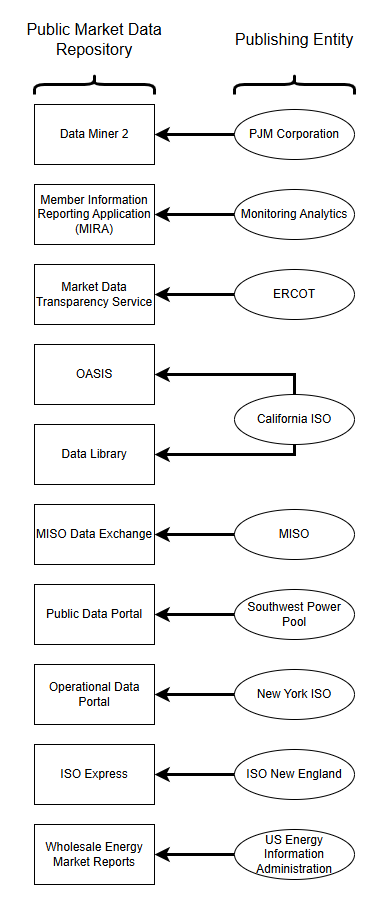
\includegraphics[scale=0.85]{graphic/market-comps.png}}
%\caption{Public Market Data Sources}
%\label{fig:market-comps}
%\end{figure}

%\section{Design Science Methodology}
%
%The roadmap of this project is based on the Design Science Research Methodology (DSRM), a research process for developing new product artifacts. The researcher chose DSRM for this project because the main research objective is to design and develop a domain-specific language for market monitors to use in their analysis.

%Data and information quality problems exist today in the market monitoring body of knowledge that a DSL-based system can help address: 

%\begin{enumerate}
%    \item {Analysts in different teams that arrive at different values when trying to quantify metrics (market impact, for example)}
%    \item {Lack of robust metadata assets such as data dictionaries and well-defined data stewardship roles}
%    \item {Lack of a mature change management program for software (which, in turn, can impact report reproducibility) }
%    \item {A lack of full automation and meta-automation, causing analysts to spend time performing tedious ETL and archival tasks}
%\end{enumerate}

%Domain-specific languages are powerful models for allowing users to systematically solve problems within a specific domain. As was determined in this literature review, DSLs have only had limited exposure in electricity markets (and even less exposure in market monitoring). This discovered gap in existing research, complemented by the DQ and IQ issues stated in this review, serves as the inspiration for this project. Figure \ref{fig:dsrm} provides more detail on the planned use of design science within this project\footnote{See Appendix \ref{appendix:C} for a schedule of the milestones and expected completion timeline for this project.}.

%\begin{figure}[h]
%\centering
%\fbox{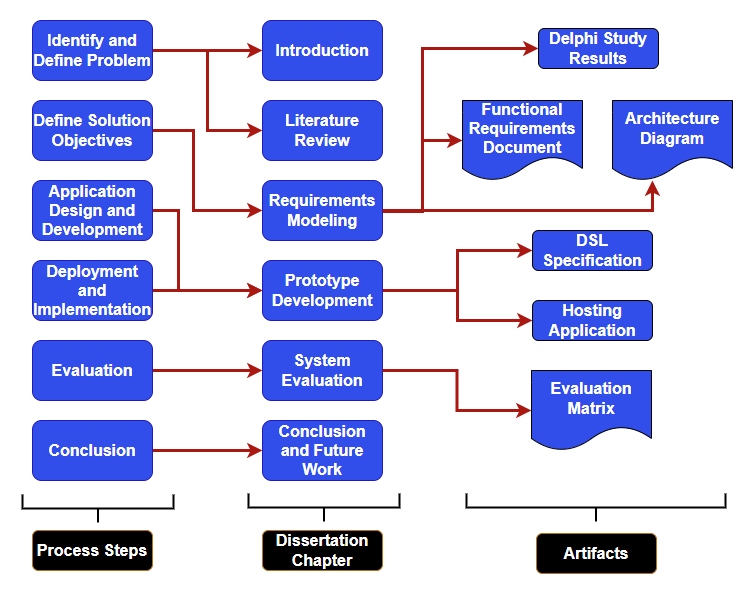
\includegraphics[scale=0.65]{graphic/dsrm_updated_20250819.png}}
%\caption{Design Science Research Methodology for this Dissertation}
%\label{fig:dsrm}
%\end{figure}

%\subsection{Proposed Investigation}

%In \textit{What Design Science Is Not (2008)}, Baskerville states that one view of design science is to be \textit{generative}. That is, design science leads to the generation of artifacts that then influence the formulation of a theory \cite{design-science-is-not}. This prospect of generativity seems to indicate that a design can be updated based upon empirical evidence. Due to this idea, the researcher chose to employ a Delphi study (as the methodology for gathering expert sentiment) to influence the design of the DSL prototype discussed in this dissertation. The following chapter discusses the setup, conduct, and results of a Delphi study employed in market monitoring. It then explains how the results of this study influenced the design and requirements document for the prototype system.

%Overall, the investigation methodology for this dissertation is composed of five (5) main components. These components include 1) a literature review, 2) a Delphi study to gather opinion and synthesize system requirements, 3) a system architecture design, 4) development of the prototype system (and associated tooling and documentation), and 5) an evaluation discussion to determine to what degree the resultant software honors the system requirements.

%\subsection{Limitations of this Research}

%The scope of work proposed in this dissertation is limited to the objectives outlined in the Proposed Investigation section. Specifically, it shall ultimately evaluate how well the developed prototype functions as a \textit{minimal viable product} (MVP) for energy market analysis.

%The proof-of-concept prototype discussed in this dissertation \textbf{is not intended to be a production-ready system}. It is also not expected to be used in a live scenario for market monitors to immediately put into service in support of decision making. The data ingested into the prototype will be based on realistic data scraped from public data systems shown in Appendix \ref{appendix:D}. The evaluation of this system will be based on a matrix (mapping back to the functional requirements document) that "scores" how well the functionality of the prototype supports the intended requirements.

%Further system optimization, bug fixes, scalability concerns, and use in live market monitoring scenarios are all currently considered "out of scope" for this dissertation and are reserved for future work. The author, however, may pursue future enhancements to this system as separate research endeavors.
